\documentclass[a4paper,12pt]{report}
%\documentclass[twoside]{article}
%\usepackage{extsizes}
\usepackage{cmap}
\usepackage[utf8]{inputenc} %Кодировка файла 
\usepackage[T2A]{fontenc} %корректное отображение русских шрифтов
\usepackage[english, russian]{babel} %переносы слов
\usepackage{fancyvrb}
\usepackage{lmodern}

%for lcov
\usepackage{lscape} %landspace
\usepackage{float}
\usepackage{tabu}
\usepackage{booktabs}
%\usepackage{xcolor}
%\definecolor{coverage_Hi}{rgb}{0, 1, 0}
%\definecolor{coverage_Med}{rgb}{1, 1, 0}
%\definecolor{coverage_Lo}{rgb}{1, 0, 0}
%\definecolor{cov_cov}{rgb}{0.9,0.9,1}
%\definecolor{cov_diff}{rgb}{1,1,0.5}
%\definecolor{cov_nocov}{rgb}{1,0.5,0.5}
%\definecolor{cov_nop}{rgb}{0.95,0.95,0.95}
\usepackage{listings}
\usepackage{picture}

\usepackage{graphicx}

%\linespread{1.3}
\renewcommand{\rmdefault}{ftm}
%\frenchspacing

%TimeNewRoman
%\usepackage{fontspec}
%\setmainfont[Mapping=tex-text]{Times New Roman}

%Поля
\usepackage{geometry}
\geometry{left=3cm}
\geometry{right=1.5cm}
\geometry{top=2.4cm}
\geometry{bottom=2.4cm}

\usepackage{verbatim}
\usepackage{spverbatim}
\renewenvironment{lstlisting}{\spverbatim}{\endverbatim}

%\renewcommand{\labelenumii}{\arabic{enumi}.\arabic{enumii}.} %стиль нумерованных списокв

\usepackage[parentracker=true,%
  backend=biber,%
  language=auto,%
  autolang=other,%
  %citestyle=gost-numeric,%
  defernumbers=true,%
  %bibstyle=gost-numeric,%
]{biblatex}
\addbibresource{bibliography.bib}

%НАСТРОЙКИ ДЛЯ DOXYGEN

\usepackage{longtable}

\usepackage{fixltx2e}
\usepackage{calc}
\usepackage{doxygen}
\usepackage[export]{adjustbox} % also loads graphicx
\usepackage{makeidx}
\usepackage{multicol}
\usepackage{multirow}
\PassOptionsToPackage{warn}{textcomp}
\usepackage{textcomp}
\usepackage[nointegrals]{wasysym}
\usepackage[table]{xcolor}



% Font selection
%\usepackage[T1]{fontenc}
\usepackage[scaled=.90]{helvet}
\usepackage{courier}
\usepackage{amssymb}
\usepackage{sectsty}
\renewcommand{\familydefault}{\sfdefault}
\allsectionsfont{%
  \fontseries{bc}\selectfont%
  \color{darkgray}%
}
\renewcommand{\DoxyLabelFont}{%
  \fontseries{bc}\selectfont%
  \color{darkgray}%
}
\newcommand{\+}{\discretionary{\mbox{\scriptsize$\hookleftarrow$}}{}{}}

% Page & text layout
%\usepackage{geometry}
%\geometry{%
%  a4paper,%
%  top=2.5cm,%
%  bottom=2.5cm,%
%  left=2.5cm,%
%  right=2.5cm%
%}
\tolerance=750
\hfuzz=15pt
\hbadness=750
\setlength{\emergencystretch}{15pt}
\setlength{\parindent}{0cm}
\setlength{\parskip}{3ex plus 2ex minus 2ex}
\makeatletter
\renewcommand{\paragraph}{%
  \@startsection{paragraph}{4}{0ex}{-1.0ex}{1.0ex}{%
    \normalfont\normalsize\bfseries\SS@parafont%
  }%
}
\renewcommand{\subparagraph}{%
  \@startsection{subparagraph}{5}{0ex}{-1.0ex}{1.0ex}{%
    \normalfont\normalsize\bfseries\SS@subparafont%
  }%
}
\makeatother

% Headers & footers
\usepackage{fancyhdr}
\pagestyle{fancyplain}
\fancyhead[LE]{\fancyplain{}{\bfseries\thepage}}
\fancyhead[CE]{\fancyplain{}{}}
\fancyhead[RE]{\fancyplain{}{\bfseries\leftmark}}
\fancyhead[LO]{\fancyplain{}{\bfseries\rightmark}}
\fancyhead[CO]{\fancyplain{}{}}
\fancyhead[RO]{\fancyplain{}{\bfseries\thepage}}
\fancyfoot[LE]{\fancyplain{}{}}
\fancyfoot[CE]{\fancyplain{}{}}
\fancyfoot[RE]{\fancyplain{}{\bfseries\scriptsize Овчинников Владислав Александрович }}
\fancyfoot[LO]{\fancyplain{}{\bfseries\scriptsize Овчинников Владислав Александрович }}
\fancyfoot[CO]{\fancyplain{}{}}
\fancyfoot[RO]{\fancyplain{}{}}
\renewcommand{\footrulewidth}{0.4pt}
\renewcommand{\sectionmark}[1]{%
  \markright{\thesection\ #1}%
}

% Indices & bibliography
%\usepackage{natbib}
\usepackage[titles]{tocloft}
\setcounter{tocdepth}{3}
\setcounter{secnumdepth}{5}
\makeindex

% Hyperlinks (required, but should be loaded last)
\usepackage{ifpdf}
\ifpdf
  \usepackage[pdftex,pagebackref=false]{hyperref}
\else
  \usepackage[ps2pdf,pagebackref=false]{hyperref}
\fi
\hypersetup{%
  colorlinks=true,%
  linkcolor=blue,%
  citecolor=blue,%
  unicode%
}

% Custom commands
\newcommand{\clearemptydoublepage}{%
  \newpage{\pagestyle{empty}\cleardoublepage}%
}

\usepackage{caption}
\captionsetup{labelsep=space,justification=centering,font={bf},singlelinecheck=off,skip=4pt,position=top}



\usepackage[pdf]{graphviz}

\title{SMTP сервер\textnumero 1}
\author{(Овчинников Владислав Александрович)}

\begin{document}
	\maketitle

	\tableofcontents

	\addcontentsline{toc}{chapter}{Введение}
	\chapter*{Введение}
	Практически каждое вычислительное устройство должно обмениваться данными с другими вычислительными устройствами, среди которых можно выделить - компьютеры, серверы, маршрутизаторы и многие другие устройства, которые требуют данные извне. Система, обеспечивающая обмен между такими устройствами называется компьютерной сетью. Для функционирования компьютерных сетей используются сетевые протоколы.

	Сетевой протокол - это набор программно-реализованных правил общения компьютеров, подключенных к сети. В настоящее время стандартом стало использование стека протоколов TCP/IP.
	
	В стеке протоколов TCP/IP были выделены четыре следующих уровня передачи информации между процессами:
	
	\begin{itemize}
		\item Канальный уровень (Ethernet, PPP, HDLC) -- предназначен для передачи данных между сетевыми адаптерами в одном сегменте сети. Также может использоваться для обнаружения и, возможно, исправления ошибок, возникших на физическом уровне.
		\item Сетевой уровень (IP) -- предназначен для передачи данных между компьютерами в разных сегментах сети. Основная цель: определение пути передачи данных. Отвечает за трансляцию логических адресов в физические. 
		\item Транспортный уровень (TCP, UDP) -- предназначен для передачи данных между процессами на разных компьютерах. При этом неважно, какие данные передаются, т.е. представляет сам механизм передачи.
		\item Прикладной уровень (HTTP, SMTP) -- обеспечивает взаимодействие сети и пользователя, разрешает приложениям пользователя иметь доступ к сетевым службам, таким как обработчик запросов к базам данных, доступ к файлам, пересылке электронной почты, просмотру веб-страниц и т.д.
	\end{itemize}

	В данной курсовой работе рассматривается разработка SMTP-клиента. Simple Mail Transfer Protocol (SMTP) - это широко используемый сетевой протокол, предназначенный для передачи электронной почты в сетях TCP/IP. SMTP впервые был описан в RFC 821. Последнее обновление в RFC 5321 включает масштабируемое расширение - ESMTP. Протокол SMTP предназначен для передачи исходящей почты с использованием порта TCP 25.

	Целью курсовой работы является реализация SMTP-клиента (как части MTA), обеспечивающего удаленную доставку и поддерживающего очереди сообщении. Вариант лабораторной работы подразумевает реализацию многопоточного SMTP-клиента с использованием вызова pselect.

	\chapter{Аналитический раздел}
	\section{Основные понятия протокола SMTP}
	В рамках курсовой работы требовалось разработать SMTP-клиент как часть MTA. Перед разработкой архитектуры был проведен анализ предметной области, связанной с решением поставленной задачи. Был рассмотрен SMTP-протокол, MTA, DNS.

	SMTP (Simple Mail Transfer Protocol) - протокол передачи сообщений с компьютера на почтовый сервер для доставки конечному получателю. Этот протокол обеспечивает перенаправление почтовых сообщений с помощью записей типа MX (или записей программы обмена электронной почтой) и записей типа A (или записей сервера в системе DNS), форматирование почтовых сообщений и установление сеансов между почтовыми клиентами и почтовыми серверами. В протоколе SMTP в качестве транспортного протокола обычно используется TCP, но могут применяться и другие протоколы, как определено в документе RFC 821.

	Обмен данными в рамках SMTP строится по принципу двусторонней связи, которая устанавливается между отправителем и получаетелем почтового сообщения. При этом отправитель инициирует соединение и посылает запросы на обслуживание, а получатель - отвечает на эти запросы. Фактически, отправитель выступает в роли клиента, а получатель - сервера. Канал связи устанавливается непосредственно между отправителем и получателем сообщения.

	Протокол SMTP не несет никакой ответственности за прием почты. В спецификации этого протокола не определены способы настройки почтовых ящиков для отдельных пользователей, а также не упоминаются какие-либо иные задачи (такие как аутентификация), которые должны быть решены при приеме электронной почты. В этой спецификации просто указано, как должна осуществляться передача электронной почты от отправителя к получателю.

	Основная задача протокола SMTP заключается в том, чтобы обеспечивать передачу электронных сообщений. Для работы через протокол SMTP клиент создает TCP-соединение с сервером через порт 25. Затем клиент и SMTP-сервер обмениваются информацией пока соединение не будет закрыто или прервано. Основной процедурой в SMTP является передача почты (Mail Procedure). Далее идут процедуры Mail Forwarding, проверка имен почтового ящика и вывод списка почтовых групп. Самой первой процедурой является открытие канала передачи, а последней - его закрытие.

	MTA (Mail Transfer Agent) - самостоятельное, минимально достаточное для приема и отправки электронной почты программное обеспечение. Важнейшей частью почтового сервера является MTA (Mail Transfer Agent - агент пересылки почты), в задачи которого входит прием и передача почты.

	MTA работает по протоколу SMTP и его одного достаточно для создания системы электронной почты. Работа MTA совмещает в себе одновременно функции внешней и локальной доставки и получения почты. MTA, получая письмо, помещает его в почтовый ящик пользователя на своем сервере, к которому последний должен получить доступ.

	MDA (Mail Delivery Agent) - это агент доставки почты, его задача по запросу почтового клиента передать ему почту из почтового ящика на сервере. MDA может работать по протоколам POP3 (Post Office Protocol v3) или IMAP (Internet Message Access Protocol), в ряде случаев для "общения" почтового клиента и агента доставки могут применяться собственные протоколы, обладающие расширенной функциональностью, например MAPI (Messaging Application Programming Interface) в Exchange Server.

	MTA (Mail Transfer Agent - агент пересылки почты) - отвечает за пересылку почты между почтовыми серверами, как правило, первый MTA в цепочки получает сообщения от MUA (почтовый агент пользователя), последний MTA передает сообщение к MDA.

	MUA (Mail User Agent) - программа, обеспечивающая пользовательский интерфейс, отображающая полученные письма и предоставляющая возможность отвечать, создавать и перенаправлять письма.

	Общение с SMTP сервером ведется при помощи команд. Команды SMTP указывают, какую операцию хочет произвести клиент. Команды состоят из ключевых слов, за которыми следует один или более параметров, Ключевое слово состоит из 4-х символов и разделено от аргумента одним или несколькими пробелами. Каждая команда заканчивается символами CRLF. Обычный ответ SMTP-сервера состоит из номера ответа, за которым через пробел следует дополнительный текст. Номер ответа служит индикатором состояния сервера.

	\begin{itemsize}
		\item EHLO - данная команда используется для начала диалога клиента с сервером и получения расширений ESMTP, которые доступны для данного сервера.
		\item HELO - устаревшая стандартная команда SMTP для начала диалога клиента с сервером (не позволяет получать расширения ESMTP).
		\item MAIL - 
		\item RCPT
		\item DATA
		\item QUIT
		\item HELP
		\item VRFY
		\item EXPN
		\item NOOP
		\item RSET
		\item TURN
	\end{itemsize}

	\section{SMTP сеанс}
	По протоколу SMTP отправитель письма связывается с получателем при помощи командной строки и специальных каналов, роль которых обычно выполняет TCP-соединение. Любая SMTP-сессия состоит из двух ведующих компонентов: команд от клиента и соответствующих им ответов сервера. При открытой сессии обе этих составляющих обмениваются ее параметрами. Подобный обмен может включать как ноль, так и больше SMTP-операций (транзакций).
	
	Любая SMTP-транзакция представляет собой три последовательные этапа команда/ответ:
	1. MAIL from. Определяет обратный адрес. Эта переменная необходима для возвращенных писем.
	2. RCPT to. Определяет получателя текущего текстового сообщения. Команда может использоваться несколько раз, в зависимости от количества получателей.
	3. DATA. Определяется для последовательной отправки текстового сообщения. Включает в себя непосредственно содержимое письма, в отличие от оболочки. "DATA" несет в себе информацию о заголовке и теле сообщения (они разделяются пустой строкой). Ответ от сервера при передаче происходит в два этапа: на первом от отвечает конкретно на команду "DATA" (уведомление о готовности принять текстовое сообщения), а на втором - о принятии или отклонении всего письма в конце последовательности данных.

	Любой SMTP-сервер выполняет несколько функций. Одной из них является проверка правильности настроек и выдача разрешения компьютеру, который пытается отправить электронное письма. Другая функция состоит в отправке исходящих писем на указанный адрес с последующей проверкой доставки. В качестве задачи, которую необходимо решить в рамках данной курсовой работы, является реализация функции отправки исходящих писем, т.е. реализация SMTP-клиента как части MTA.


	\section{Архитектура взаимодействия клиента с сервером}

        ...


	\begin{figure}[H]
		\centering
		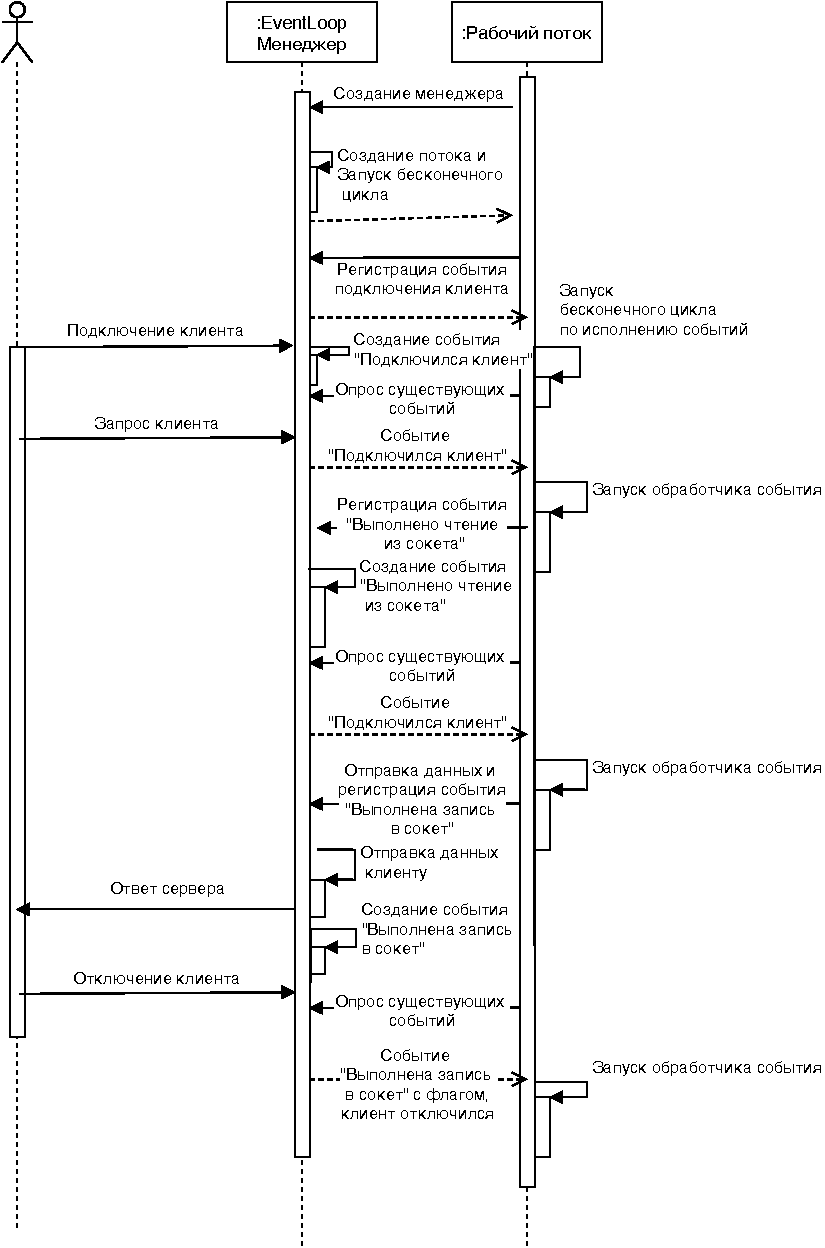
\includegraphics[width=0.8\textwidth]{./resource/SequenceDiagram_EventLoop.pdf}
		\caption{ Диграмма последовательности взаимодействия клиента с сервером, описывающая подключение клиента, который отправлет запрос, ожидает ответ, а потом отключается.} 
		\label{fig:EventLoopSequence}
	\end{figure}


 	\chapter{Конструкторский раздел}

 	\section{Разработка SMTP-клиента}
    
    	\begin{figure}[h]
		\centering
		\includegraphics[width=\textwidth]{./include/smtp_fsm.pdf}
		\caption{Конечный автомат протокола SMTP для клиента}
		\label{fig:smtp_fsm}
	\end{figure}
     
    	\section{Описание формата хранения писем в файловой системе}
    	
	Для хранения почты, получаемой сервером посрдеством почтовой транзакции, используется файловая система. Используемая струтктура каталогов взята из спецификации \textit{MAILDIR}, которая описана в [???]. Формат maildir имеет следующую структуру каталогов:
    	\begin{verbatim}
        	- maildir
        		-user1
            			-cur
            			-tmp
            			-new
        		-user2
            			-cur
            			-tmp
            			-new
    	\end{verbatim}
    Где maildir\_root - кореньевая папка. user\_path, user2\_path - каталоги пользователей текущей почтовой службы. cur, tmp, new - папки содержащие письма. 
    new - сюда попадают письма новые письма, которые пользователь не прочитал. cur - письма просмотренные пользователем. tmp - пиьсма находящиеся на стадии доставки, необходимость этой папки заключается в том, что запись данных в файл не является атомарной операцией. Если этой папки не будет то при создании файла, например в папке new, может произойти так, что программа для чтения локальной почты, попытается открыть этот новый файл, а программа доставки почты еще не успела туда записать данные. По этому используется каталог tmp для исключения таких случаев. Пока данные записываются в файл, тот находится в папке tmp, как только письмо полностью записано в файл, то программа доставки писем перенсит этот файл в каталог new.
    
    При создании новых файлов писем, им необходимо даватб имена. Для создания уникального имени формат MAILDIR трактует слудющие правила:
    \begin{verbatim}
        <pid><sender_mailbox><timestamp><random_value>
    \end{verbatim}
    Где <pid> - идентификатор процесса, выполняющий доставку почты; <sender\_mailbox> - адрес электронной почты отправителя письма;  <timestamp> - время UNIX; <random\_value> - случайное целое число.
    
    Поскольку формат MAILDIR разработан для доставки локальной почты, а по заданию необходимо обрабатывать и глобальную почту (почту адресованную пользователям на других серверах), то формат MAILDIR был модифицирован следующим образом: 
        
    \begin{verbatim}
        - maildir
                -user1
                        -cur
                        -tmp
                        -new
                -user2
                        -cur
                        -tmp
                        -new
                .OTHER_SERVERS
                        -domain_server1
                                -tmp
                                -letter1
                                -letter2
                        -domain_server2
                                -tmp
                                -letter1
                                -letter2
    \end{verbatim}

    Модификация maildir добавляет папку \textit{.OTHER\_SERVERS}, в которой слкадываются все письма, приходящие на данный сервер, но адресованные пользователям других почтовых служб. папки \textit{.OTHER\_SERVERS/tmp} и  \textit{.OTHER\_SERVERS/new} имеют теже самые назначения, что и папки для пользователей. Папка \textit{.OTHER\_SERVERS/cur} отсутствует, так как после того как письма из папки \textit{.OTHER\_SERVERS/new} будет доставлено другому серверу будет удалена. Так же изменен формат создания уникального имени файла:
    \begin{verbatim}
        <timestamp>_<random_value>
    \end{verbatim}
    Использую такой формат, нельзя определить по файлу от кого письмо и кому адресовано, по этому при записи письма в \textit{.OTHER\_SERVERS} к телу письма дописываются дополнительные заголовик, с помощью которых отправляющая программа сможет определить адресата и адресанта:
    \begin{verbatim}
        X-Postman-From: <mailbox>
        X-Postman-Date: <timestamp>
        X-Postman-To: <mailbox> [, <mailbox> [...]]
        <пустая строка (\r\n)>
        <тело письма полученное во время почтовой транзакции>
    \end{verbatim}
    
    Обработка данной структуры в файловой системы реаизовано с помощью класса \textit{maildir}. Дописыване дополнительных заголовков реализовано в обработчике почтовой транзакции, а не внутри класса \textit{maildir}.

\section{Логика программы}

	\begin{figure}[H]
		\centering
		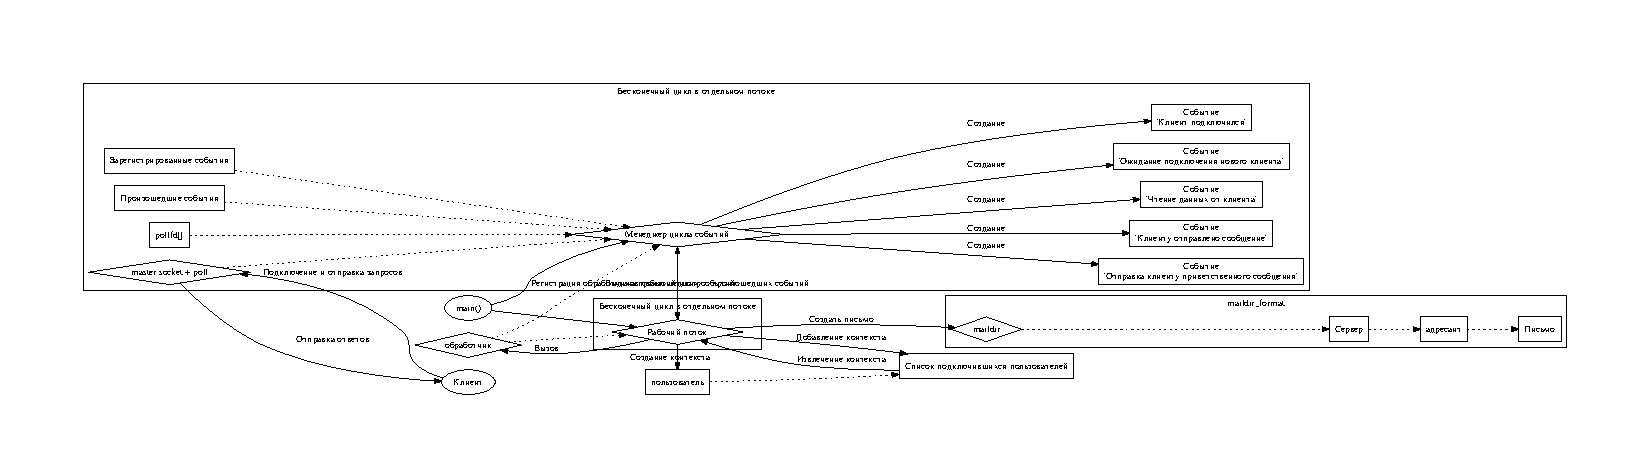
\includegraphics[width=\textwidth]{./resource/logic.pdf}
		\caption{Упращенная диаграмма взаимодействия модулей. EventLoop осуществлет обработку подключений. Рабоий поток осуществляет вызов обработчиков событий, которые EventLoop создает. Модуль mailidr обеспечивает сохраенние писем в файловой ситемы в соответсвующем формате} \label{fig:ProgLogic}
	\end{figure}

	Программа написана с использованием Объектно Ориентированной парадигмы, хотя язык С напрямую ее не поддерживает. Для описания объектов используются структуры, для которых принято слоедующее соглашение:
	\begin{itemize}
		\item Поле считается приватным (private) если его название начинается с префика pr или \_ (нижнее подчеркивание). Защищенные (protected) поля не используются.
		\item Функция (метод структуры) считается приватным, если его название начинается с префикса pr или \_ (нижнее подчеркивание)
	\end{itemize}
	Так же используется некоторое подобие наследования в цилке событий, которе будет описано далее.
	
	Работа программы начинается с того, что выполняется чтение конфигурационного файла, пример которого представлен в следующем листинге. 

	\VerbatimInput{../../resource/config2.cfg}

	Чтение конфигурационного файла реализовано посредством бибилотеки \textit{libconfig}. \textit{server\_config\_init} реализует логику для заполнения глобальной структуры \textit{server\_configuration} содержащая все необходимые объекты для работы сервера. 

	 После инициализации данной структуры, выполнятся создание экземпляра класса цилка событий (event_loop с помощью функции el\_init), затем создается сокет, выполняющий прослушивание порта (master_socket, функция make\_server\_socket). Далее для данного сокета выполняется регистрация обрабтчика события подключения нового клиента. (обработчик - функция handler\_accept) Регистрация выполняется для конкретного экземлпяра структуры event\_loop. Таким образом, когда клиент выоплнит подключение к серверу, будет вызван зарегистрированный обработчик, в который будет передедан экземпляр event_loop, серверный сокет и клиентский сокет. На рисунке \ref{fig:handlers} показана логика взаимодействия разных видов обработчиков между собой. Это взаимодействие существует, поскольку все событя, кроме таймеров и подключения новых клиентов являются одноразовыми и их необходимо заново регистрировать.

	 	\begin{figure}[H]
		\centering
		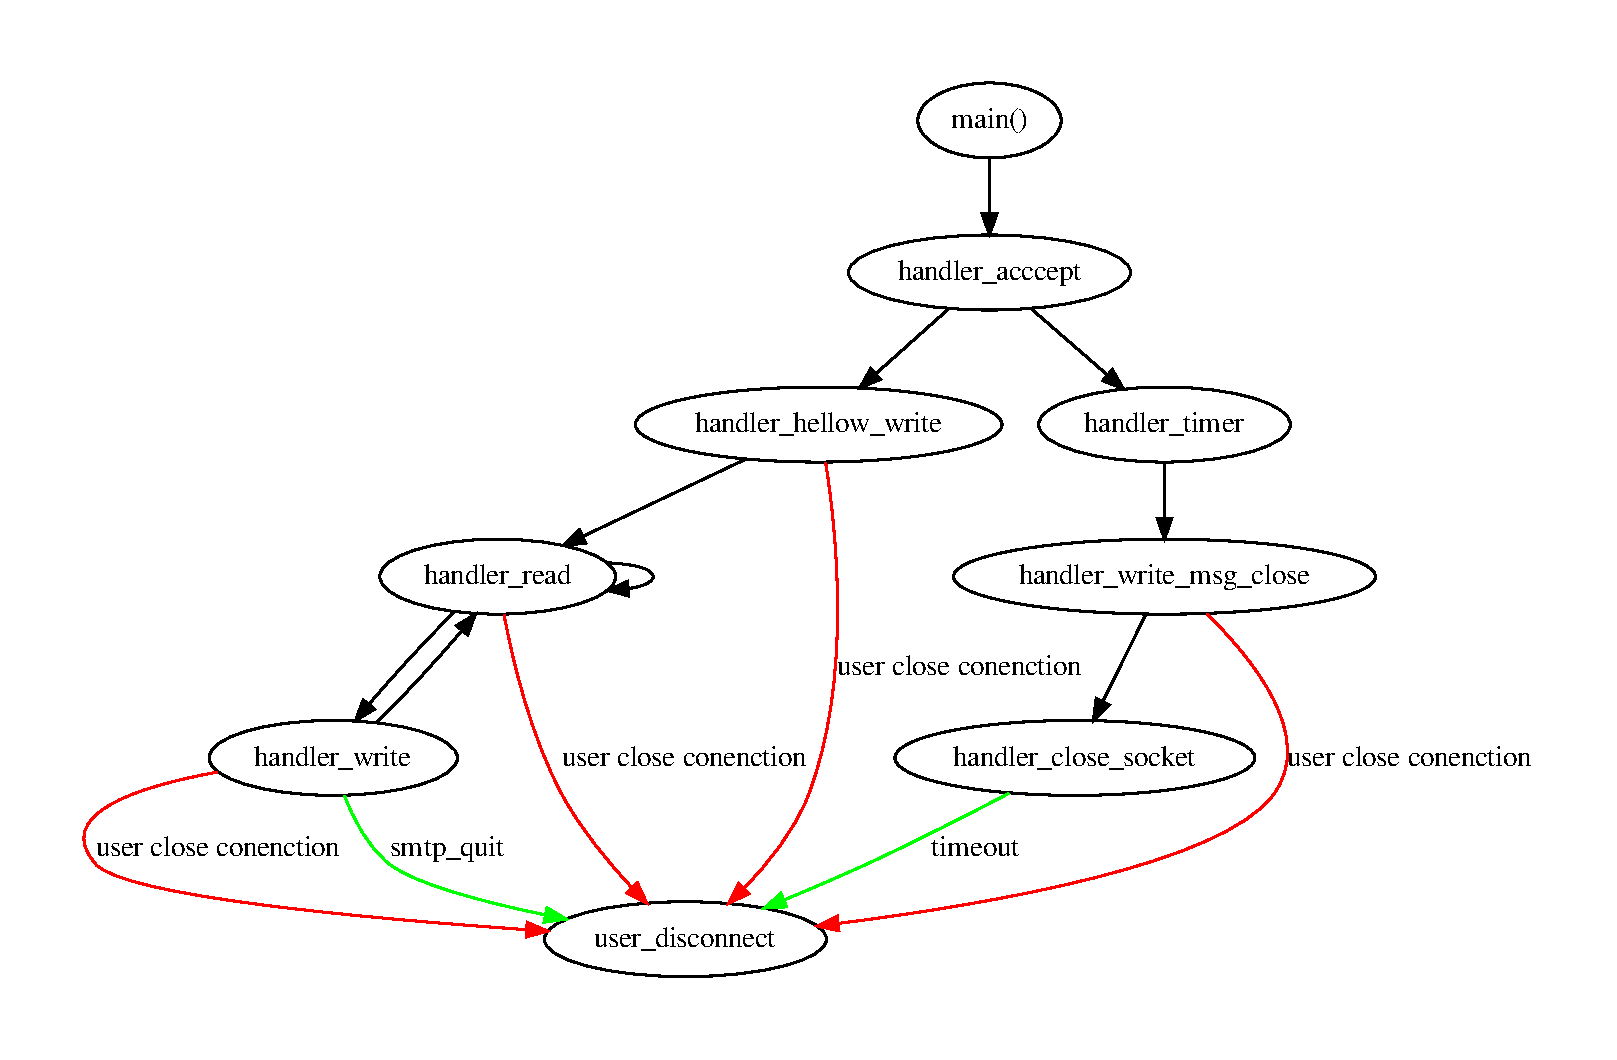
\includegraphics[width=\textwidth]{./resource/handlers.pdf}
		\caption{Псоледовательность выполнения обработчиков событий. функции main и user\_disconnet не явлются обработчиками в смыле event\_loop, а явлются началом и концом работы.  Стрелками обозначены возможные переходы во время работы. При этом две образовавшеся ветки, работают одновременно. Так как event\_loop многопоточный. Зеленая стрелка означает корректный переход в конечное состояние, а красная -- переход по возникшей ошибке} \label{fig:ProgLogic}
	\end{figure}
	Жизненый цилк взаимодействия клиента с сервером начинает с обработчика handler\_accept, который вызывается при подключении клиента к серверу. В этот момент регистрируются обработчики для отправки приветсвенного сообщения от сервера и таймер на ождинаие команд от пользователя. Левая ветка, описывает переходы между обработчиками во время передачи команд от клиента к серверу, и передачи откликов от сервера клиенту. Правая ветка следит за тем, что клиент успевая отправлть команды в зафиксированне промежутки времени. Но клиент, может выполнить отключение от сервера нарушая протокол SMTP (самостоятельно или по ошибке, такие переходы обозначены, красной линией). Завершение работы с клиентом выполняется в функции client\_disconnect, в которой выоплняется очищение всех ресурсов, выделенных во время работы с клиентом.

	\begin{figure}[H]
	\centering
	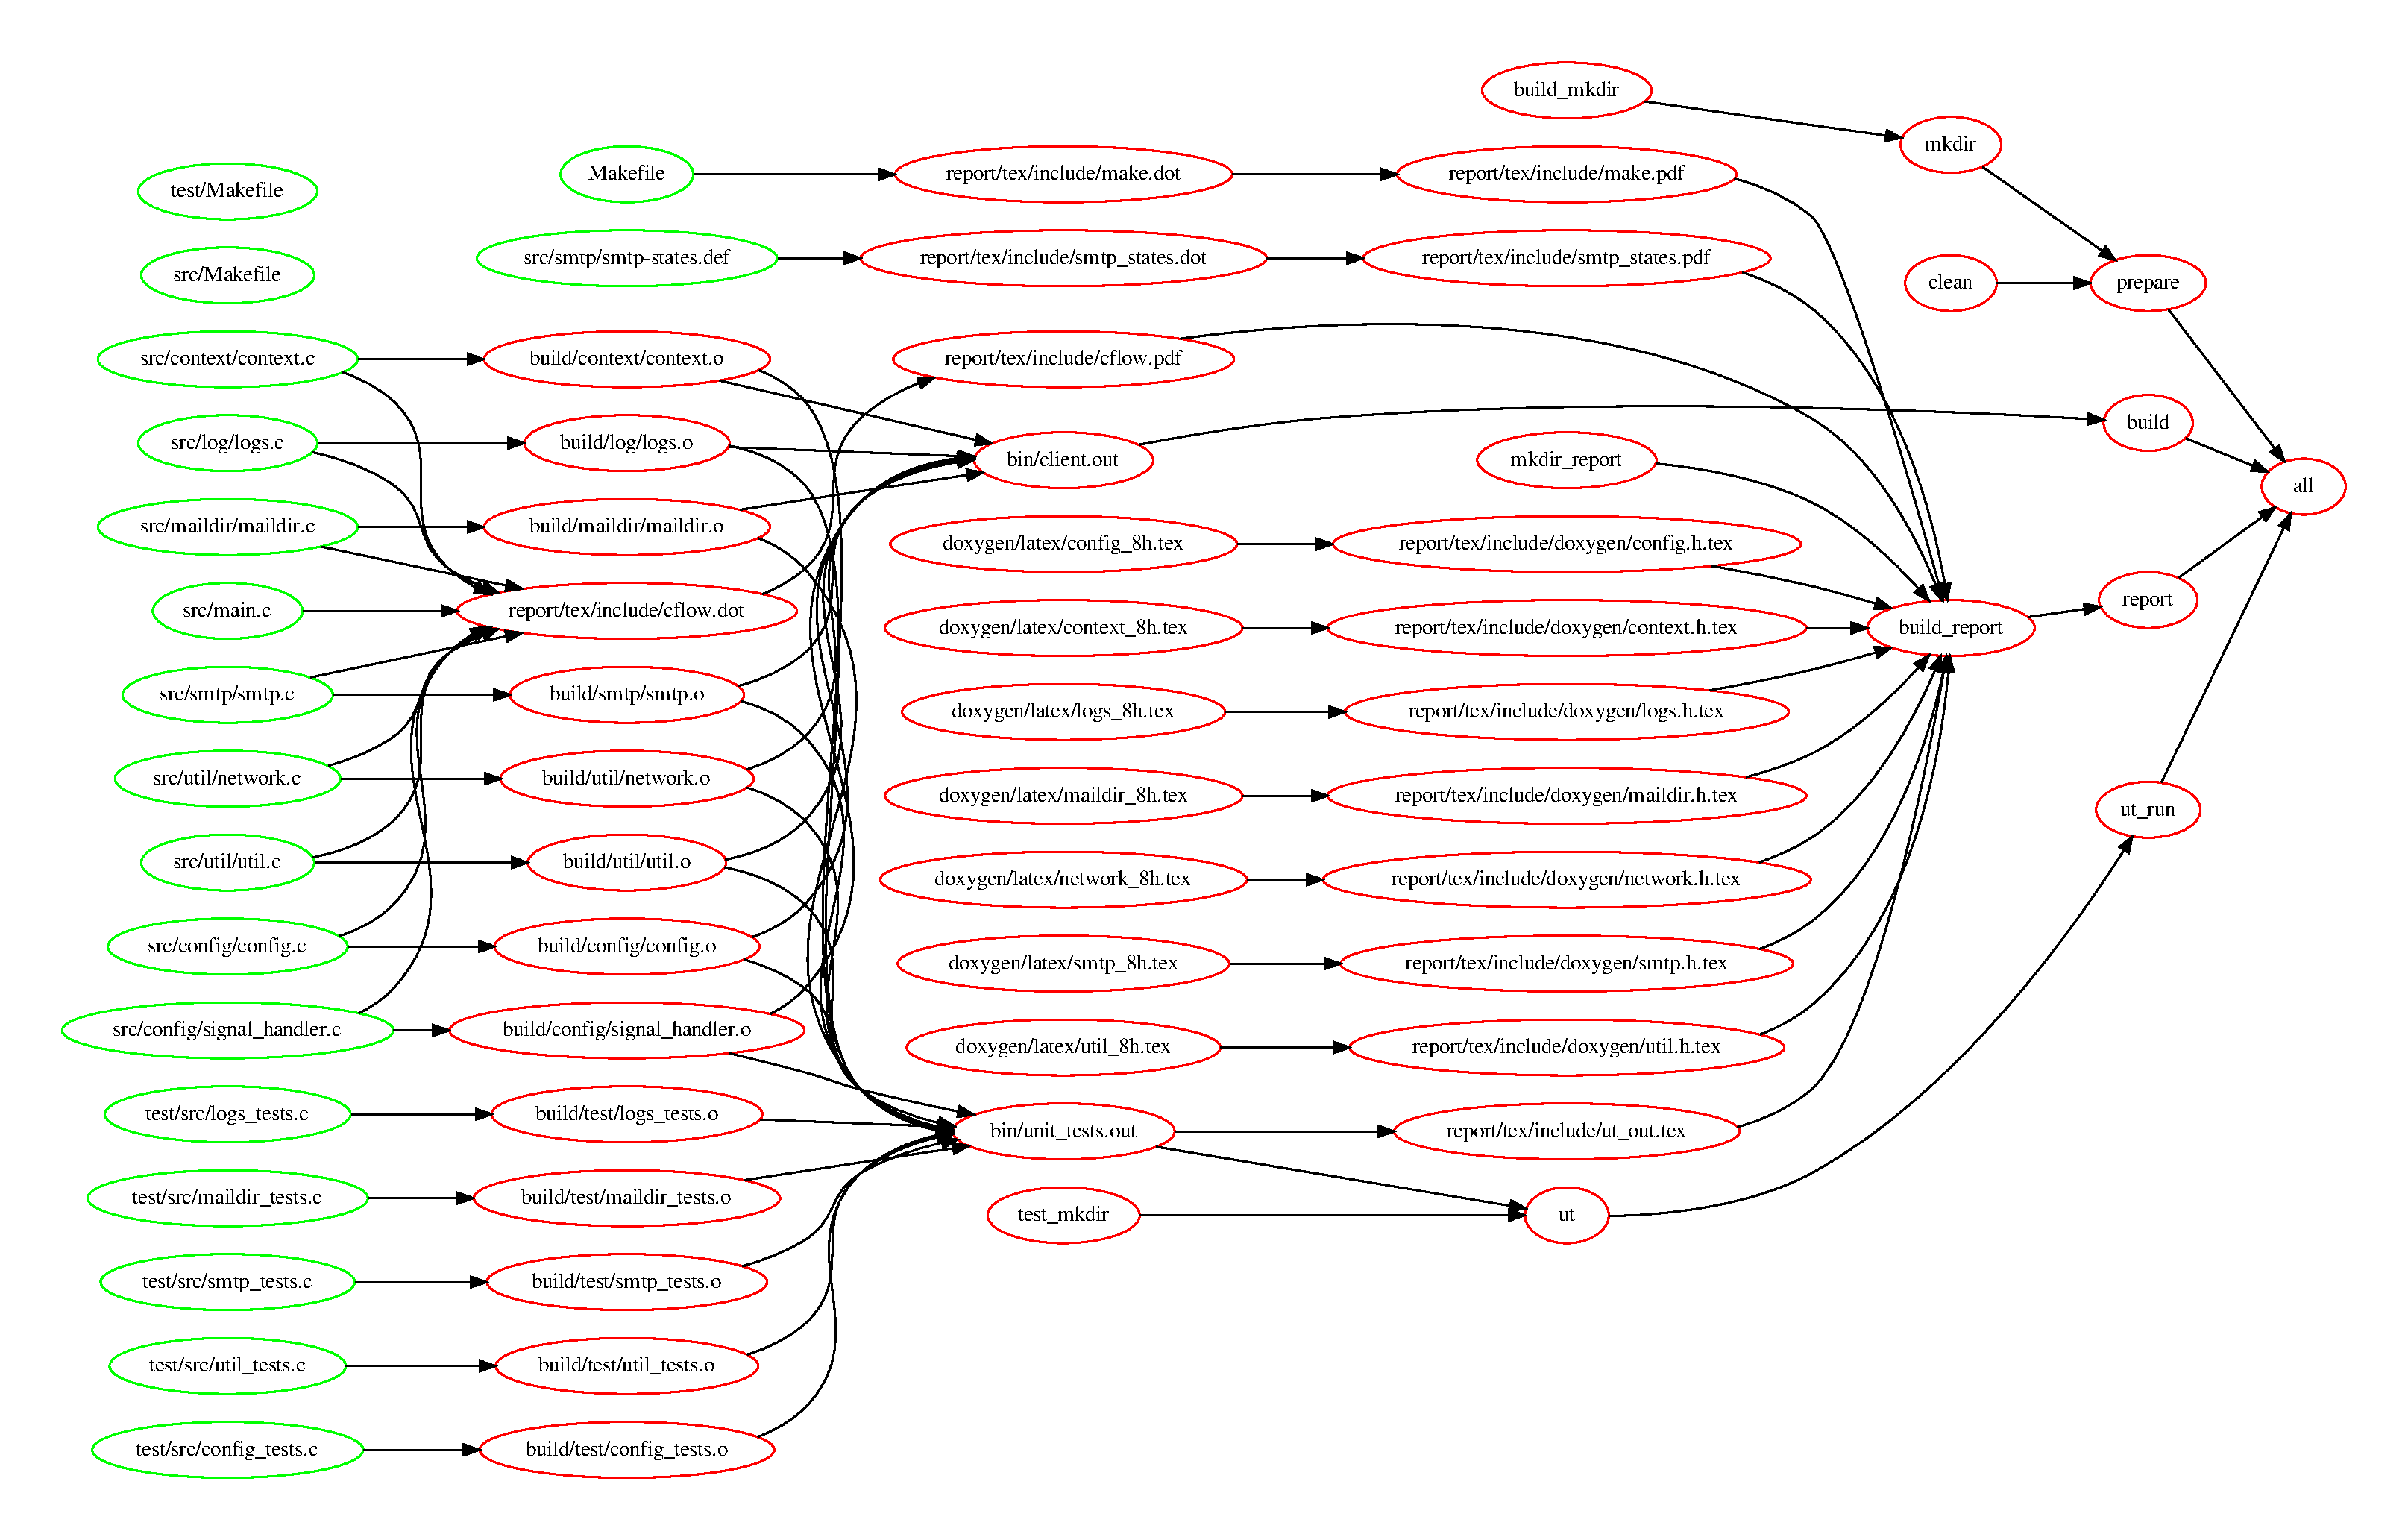
\includegraphics[width=\textwidth]{./include/make.pdf}
	\caption{Структура проекта.}
	\label{fig:make_server}
	\end{figure}

	
	\begin{figure}[H]
	\centering
	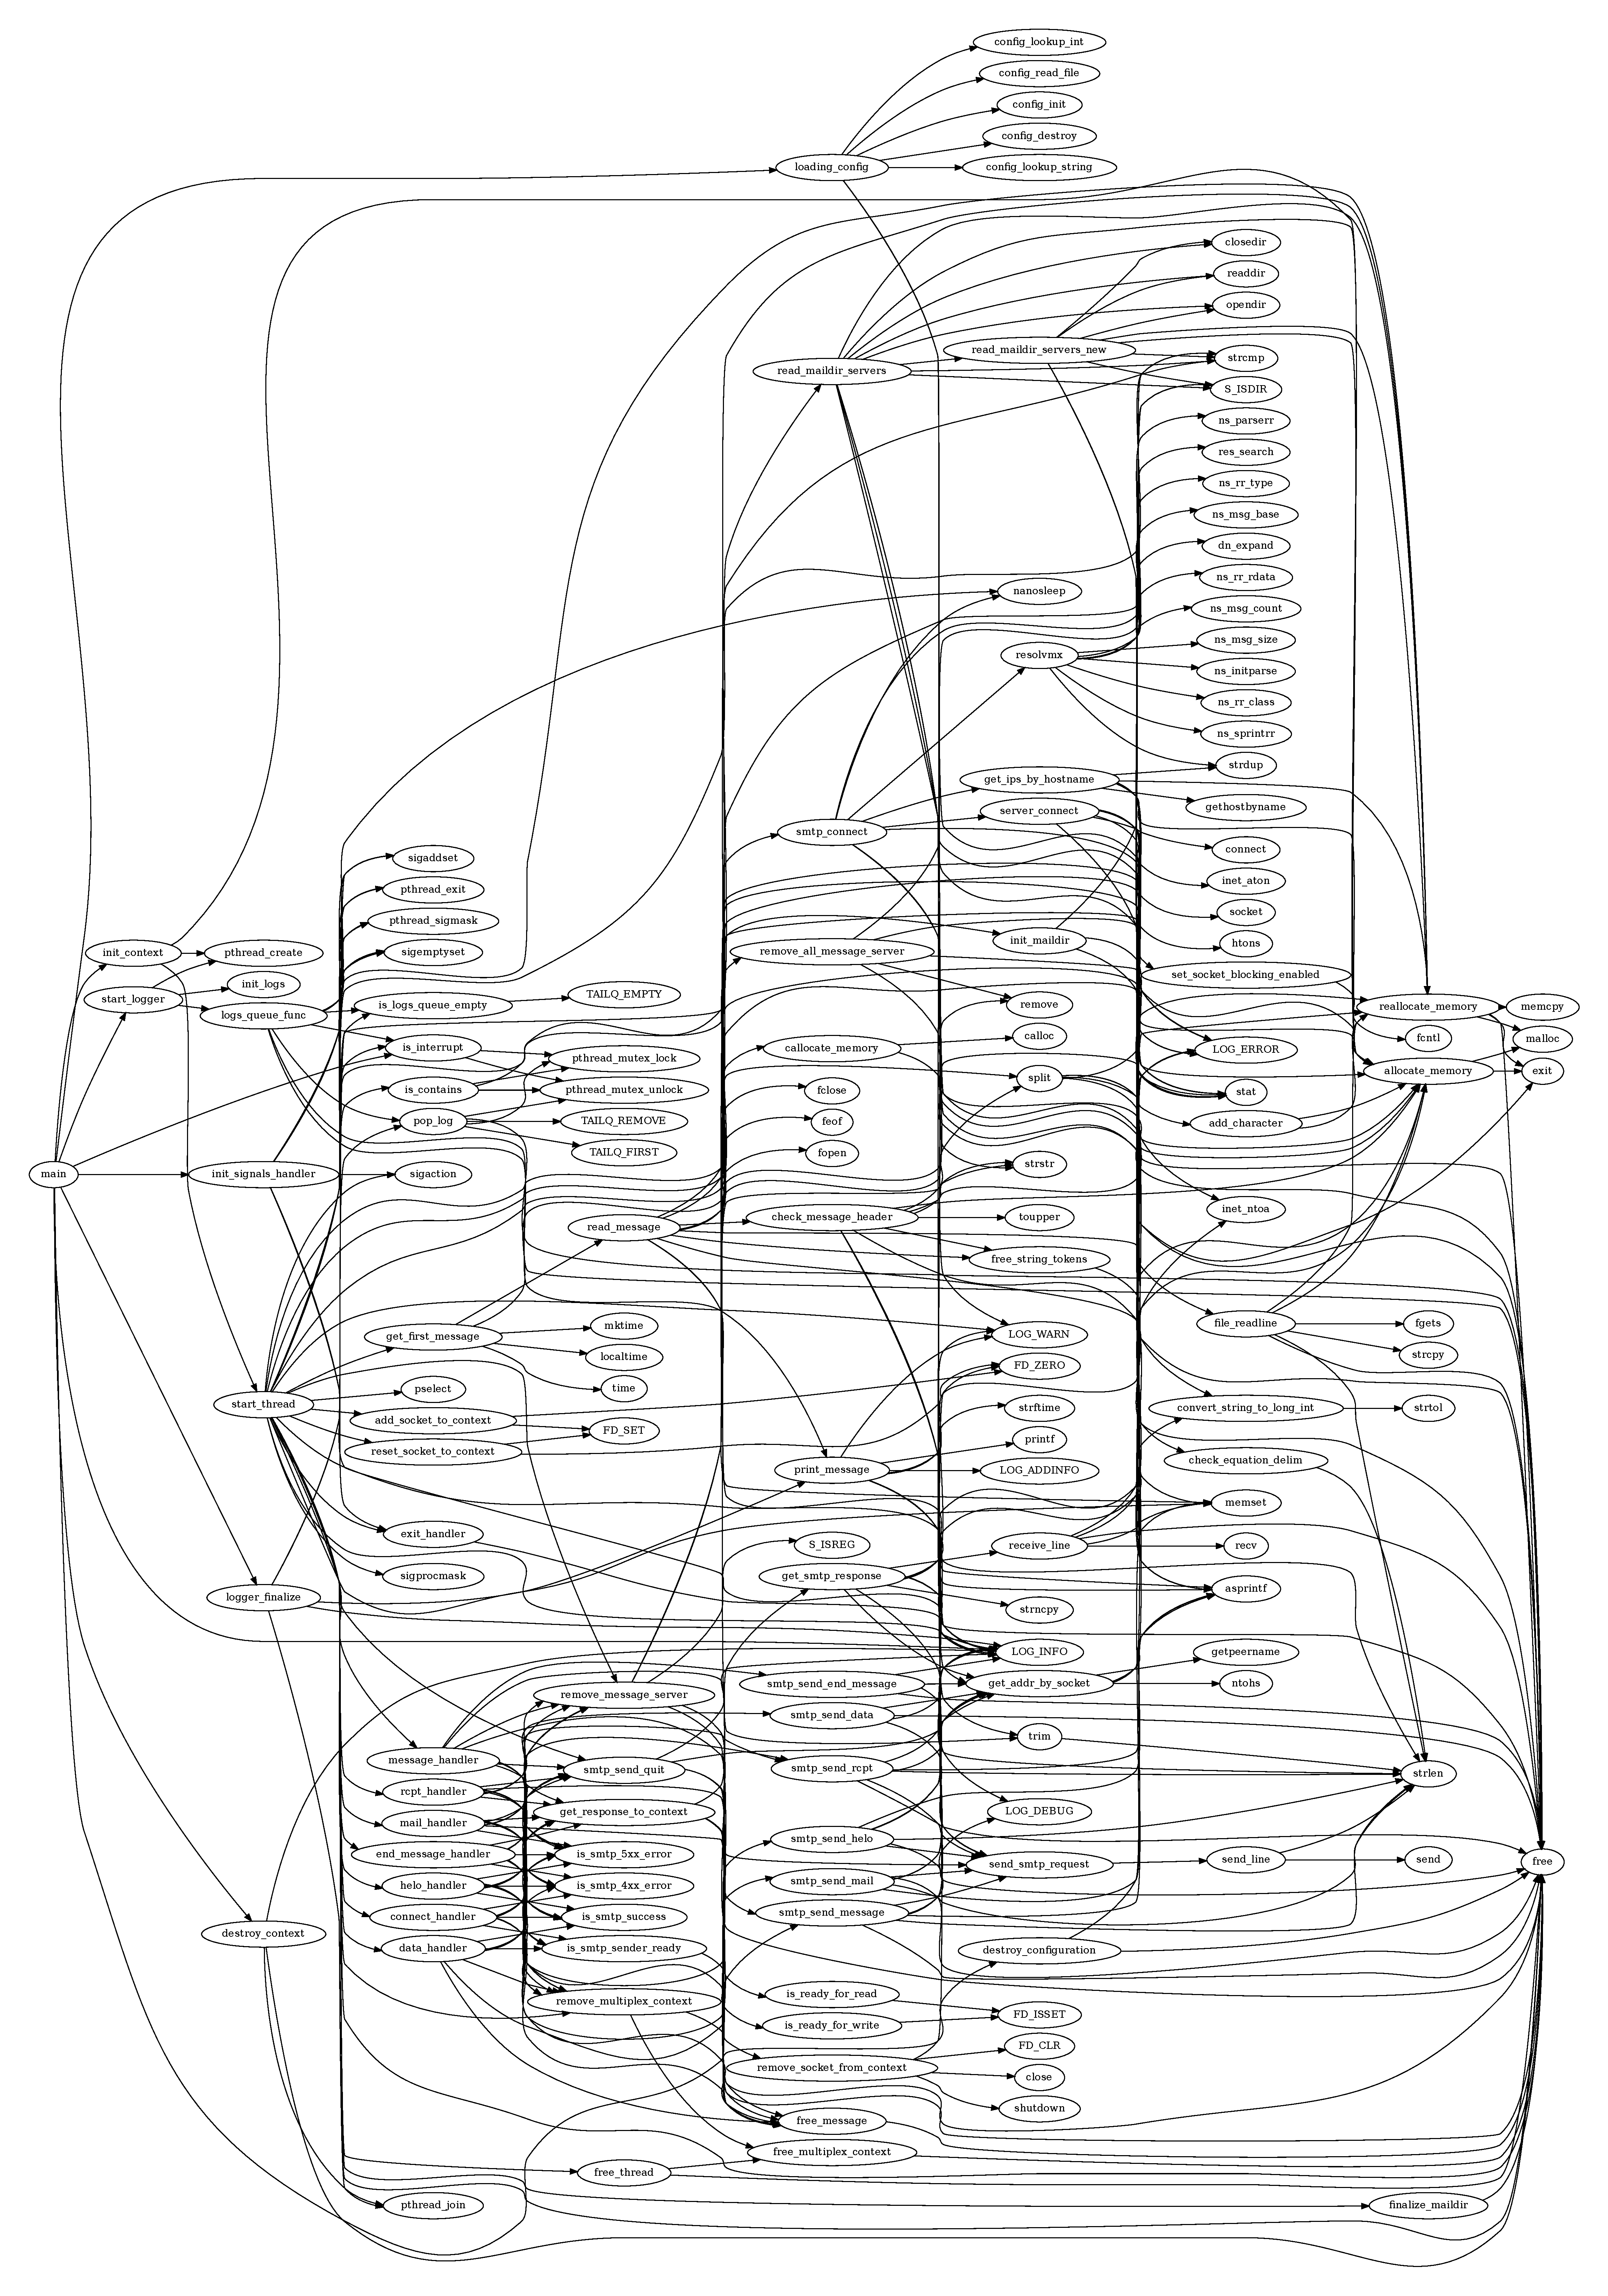
\includegraphics[width=\textwidth]{./include/cflow.pdf}
	\caption{Граф вызовов функций, который реализует всю логику.}
	\label{fig:event}
	\end{figure}



	\section{Тестирование}
		Для тестирования отдельных модулей сервера, было написаны unit-тесты
		с использованием библиотеки cunit. Резултат работы тестиованяи представлен
		в листинге 
		\VerbatimInput{./include/unit_test_out.tex}
		\VerbatimInput{./include/valgrind_out.tex}
		
		Так же было реализовано системное тестирование, на языке программирования python.
		%\begin{landscape}
		%	\input{./include/lcov/index}
		%\end{landscape}
		%Отчет по покрытию тестами не строится в  gitlab!

\section{Основные функции программы}

Данный раздел  создан с помощью программы doxygen

\input{./include/doxygen/event_loop.h.tex}
\input{./include/doxygen/smtp_state.h.tex}
\input{./include/doxygen/smtp_state.h.tex}   
\input{./include/doxygen/maildir.h.tex}
\input{./include/doxygen/maildir_server.h.tex}
\input{./include/doxygen/maildir_user.h.tex}
\input{./include/doxygen/maildir_user.h.tex}	

	\section{Список источников и литературы}
	\begin{enumerate}
		\item http://rfc.com.ru/rfc2821.htm
		\item http://rfc.com.ru/rfc1123
		\item https://www.protocols.ru/WP/rfc5322/
		\item RFC 1035 DOMAIN NAMES — IMPLEMENTATION AND SPECIFICATION  https://www.protocols.ru/WP/rfc1035/
		\item dovecot maildir https://wiki.dovecot.org/MailLocation/Maildir
		\item qmail maildir https://cr.yp.to/proto/maildir.html
	\end{enumerate}
	
	\newpage
	%\appendix
	%\section{A}\label{appendix:event_loop}
	% \begin{figure}[H]
    %\centering
  %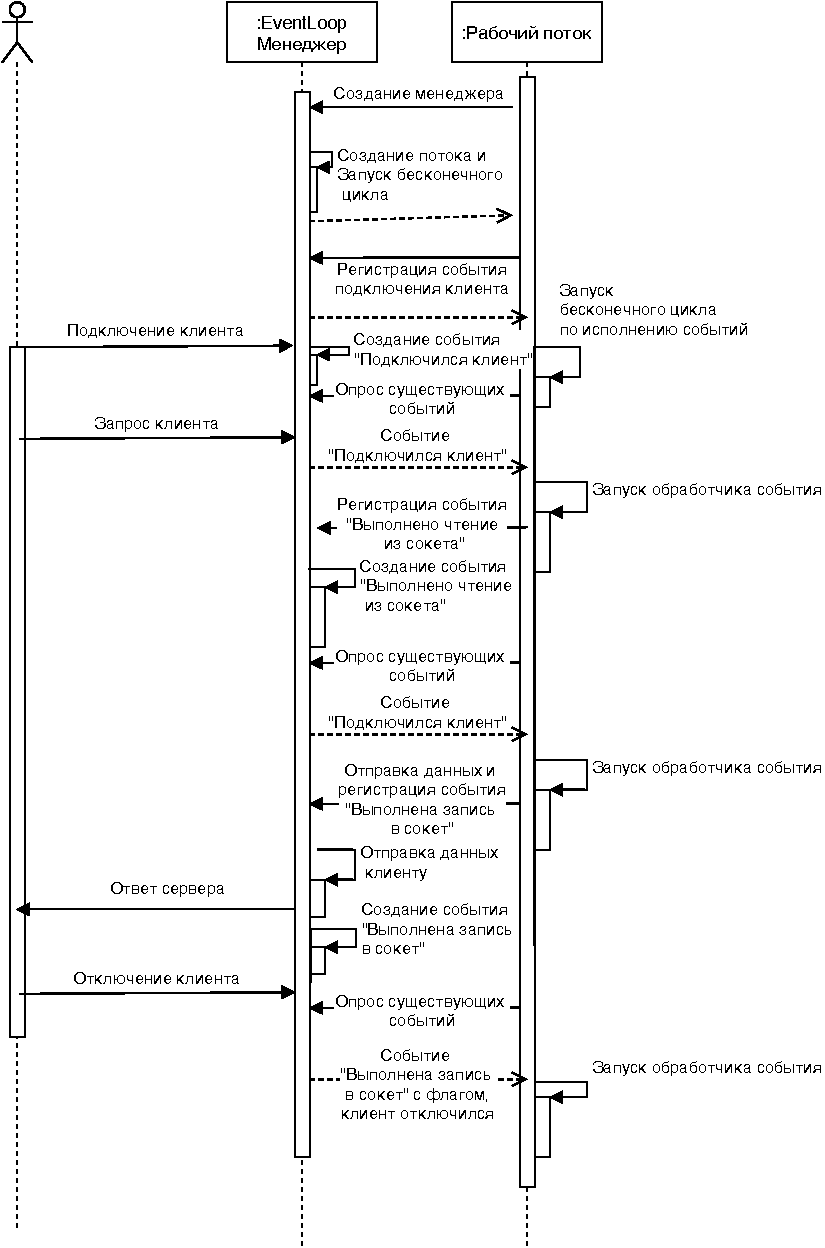
\includegraphics[scale=01]{./resource/SequenceDiagram_EventLoop.pdf}
%\end{figure}
 % Диграмма последовательности цикла событий сервера, описывающая подключение клиента, который отправлет запрос, ожидает ответ, а потом отключается. При отключении клиента, выставлется соответсвующий флаг, который обрабатывается в обработчике чтения из сокета или записи в сокет.
\end{document}
